% Титульный лист
\begin{titlepage}
\thispagestyle{empty}

\begin{center}

% ===== Верх страницы =====
\logo

% Свободное пространство до центра
\vspace{0.5cm}

% ===== Заголовок в центре страницы =====
\newcommand{\myskip}{\\}
{\bfseries\Large
ТЕХНИЧЕСКОЕ ОБСЛУЖИВАНИЕ\myskip
ЛЕГКОГО МНОГОЦЕЛЕВОГО\myskip
ГУСЕНИЧНОГО\myskip
ТРАНСПОРТЕРА-ТЯГАЧА МТЛБ\myskip
}

% Свободное пространство до низа
\vfill

% ===== Фото внизу =====

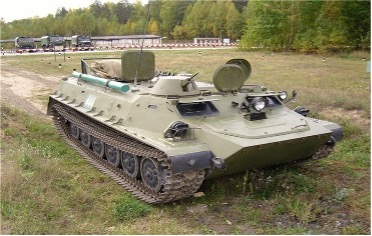
\includegraphics[width=0.95\textwidth]{src/mtlb.jpg}

\end{center}


\end{titlepage}

%====================================================
% ПУСТАЯ СТРАНИЦА 
%====================================================
\newpage
\thispagestyle{empty}
\mbox{}
\newpage

%====================================================
% ВТОРАЯ СТРАНИЦА 
%====================================================

\clearpage
% \thispagestyle{plain}

\begin{center}

\logo

\vspace{1cm}

{\Large\bfseries
Техническое обслуживание\\
легкого многоцелевого гусеничного транспортера-тягача МТЛБ
}

\vspace{1.5cm}

Учебное пособие

\vfill

\end{center}

\begin{flushright}
Рассмотрено и одобрено\\
на заседании военного учебного центра\\
Протокол №\rule{1.5cm}{0.4pt} от \rule{4cm}{0.4pt} 2026 г.\\
\end{flushright}

\vfill

\begin{center}
Санкт-Петербург
\end{center}

%====================================================
% СТРАНИЦА С АННОТАЦИЕЙ
%====================================================
\clearpage
\thispagestyle{empty}

\vspace*{\fill}
{
    % {\large\bfseries АННОТАЦИЯ} % Раскомментируйте, если нужен заголовок
    
    \noindent
    В учебном пособии рассмотрены вопросы периодичности и объема работ по техническому обслуживанию легкого многоцелевого гусеничного транспортера-тягача МТЛБ. Дано иллюстрированное сопровождение текстового материала.
    
    \medskip

    \noindent
    Учебное  пособие предназначено для студентов, проходящих военную подготовку по программам сержантов и солдат запаса, а также может быть использовано профессорско-преподавательским составом при подготовке и проведении занятий.
    
    \medskip
    
    \noindent
    Авторский коллектив: подполковник запаса Бахуревич~В.С., подполковник запаса Фирсов~О.А.
    
    \medskip
    
    \noindent
    Под общей редакцией генерал-майора запаса Глинина~В.Н.
    
    \medskip
    
    \noindent
    Авторский коллектив выражает искреннюю благодарность курсанту Гребенкину~И.А. за редакторские замечания, а также за профессиональную техническую подготовку и верстку настоящего издания.
}

\vspace*{\fill}